\newpage
\section{Actividad 2.2: HDL decodificador BCD}

\subsection{Materiales Requeridos}
\begin{itemize}
    \item Software de simulación (Xilinx ISE)
    \item Kit CPLD
\end{itemize}

\subsection{Procedimiento}

\begin{enumerate}
    \item Describir en HDL – verilog.
    \item Sintetizar y obtener el RTL en un CPLD XC9572XL.
    \item Generar el UCF
    \begin{itemize}
        \item Identifica los pines de display 7 segmentos.
        \item Identificar el transistor que activa el display a utilizar.
        \item Identificar la llave a utilizar.
    \end{itemize}
    \setlength\itemsep{0.1em} % Ajusta el espacio entre ítems
    \item Implementar el diseño.
    \item Simular.
    \item Conectar kit CPLD.
    \item Conecta la fuente de alimentación.
    \item Abrir “Manager Configuration Project”.
    \item Borrar CPLD.
    \item Cargar archivo binario *.JED.
    \item Demostrar correcto funcionamiento al realizar las diferentes pruebas utilizando distintas entradas BCD para asegurarte de que el decodificador funcione correctamente.
\end{enumerate}
\subsection{Implementación}
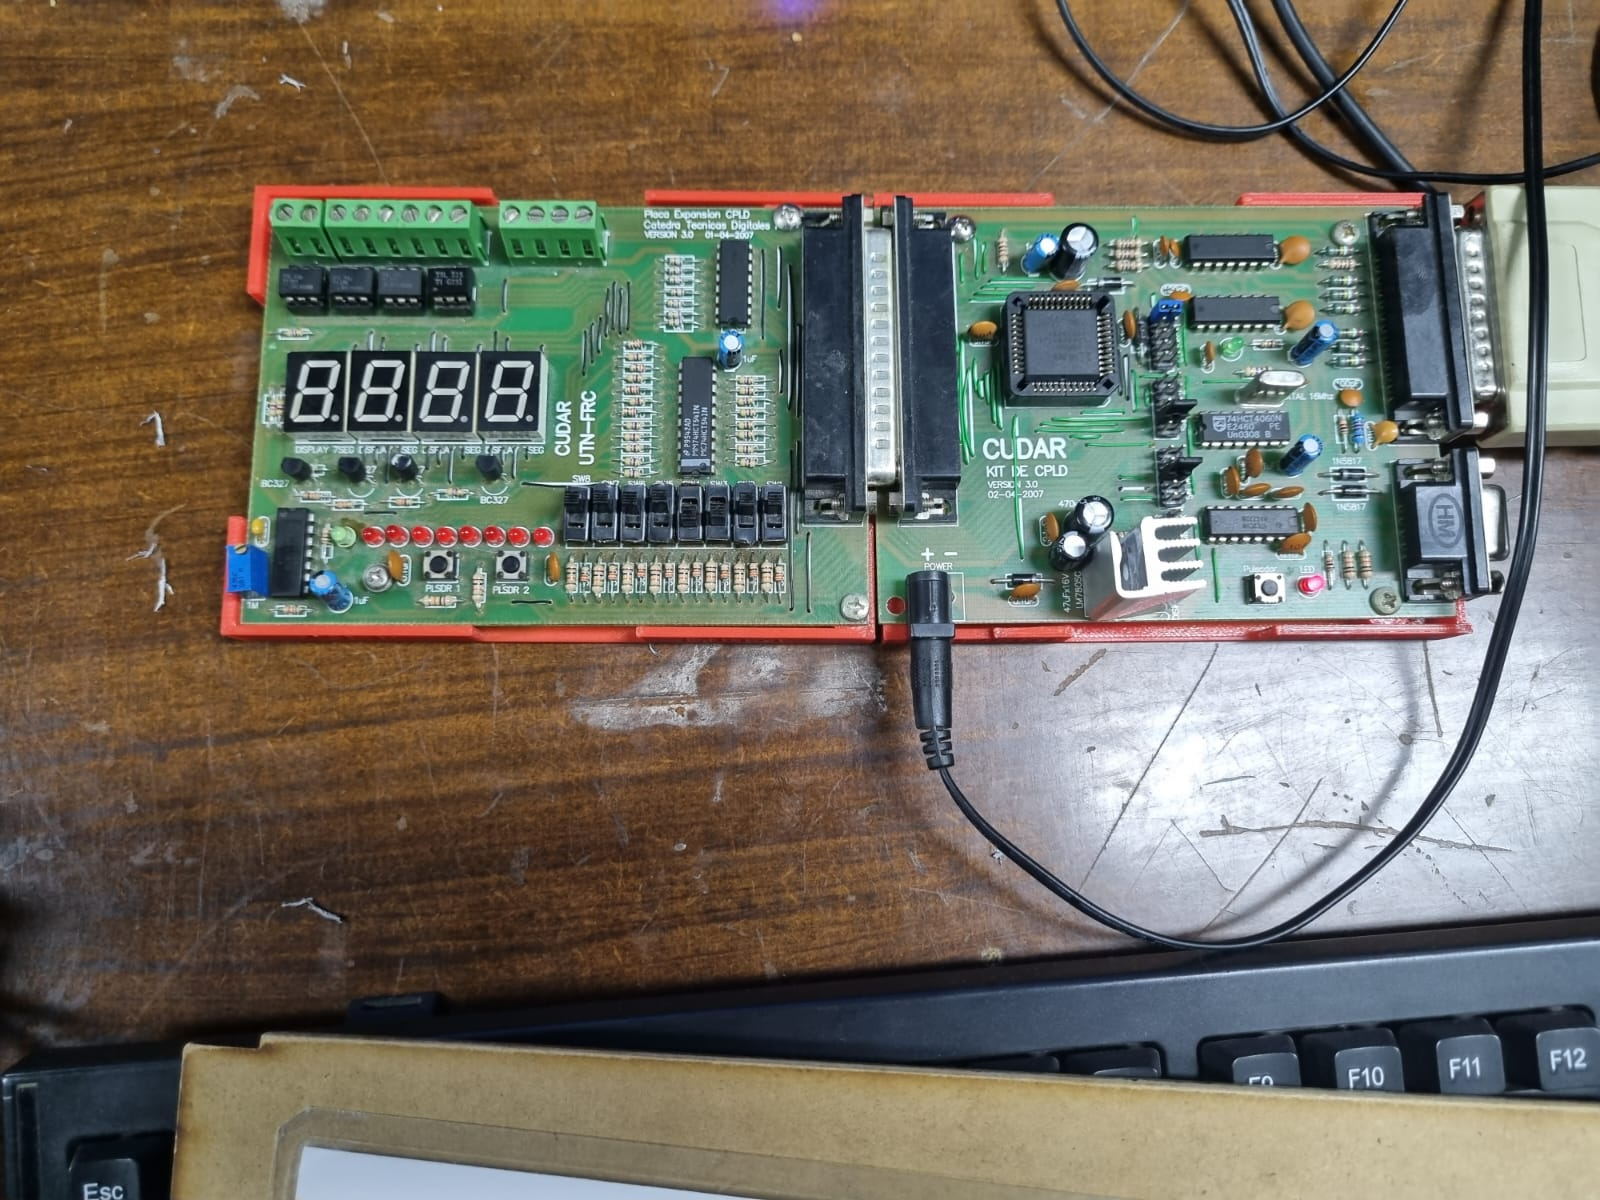
\includegraphics[width=14cm]{./imagenes/cpld.jpeg}
\paragraph{}
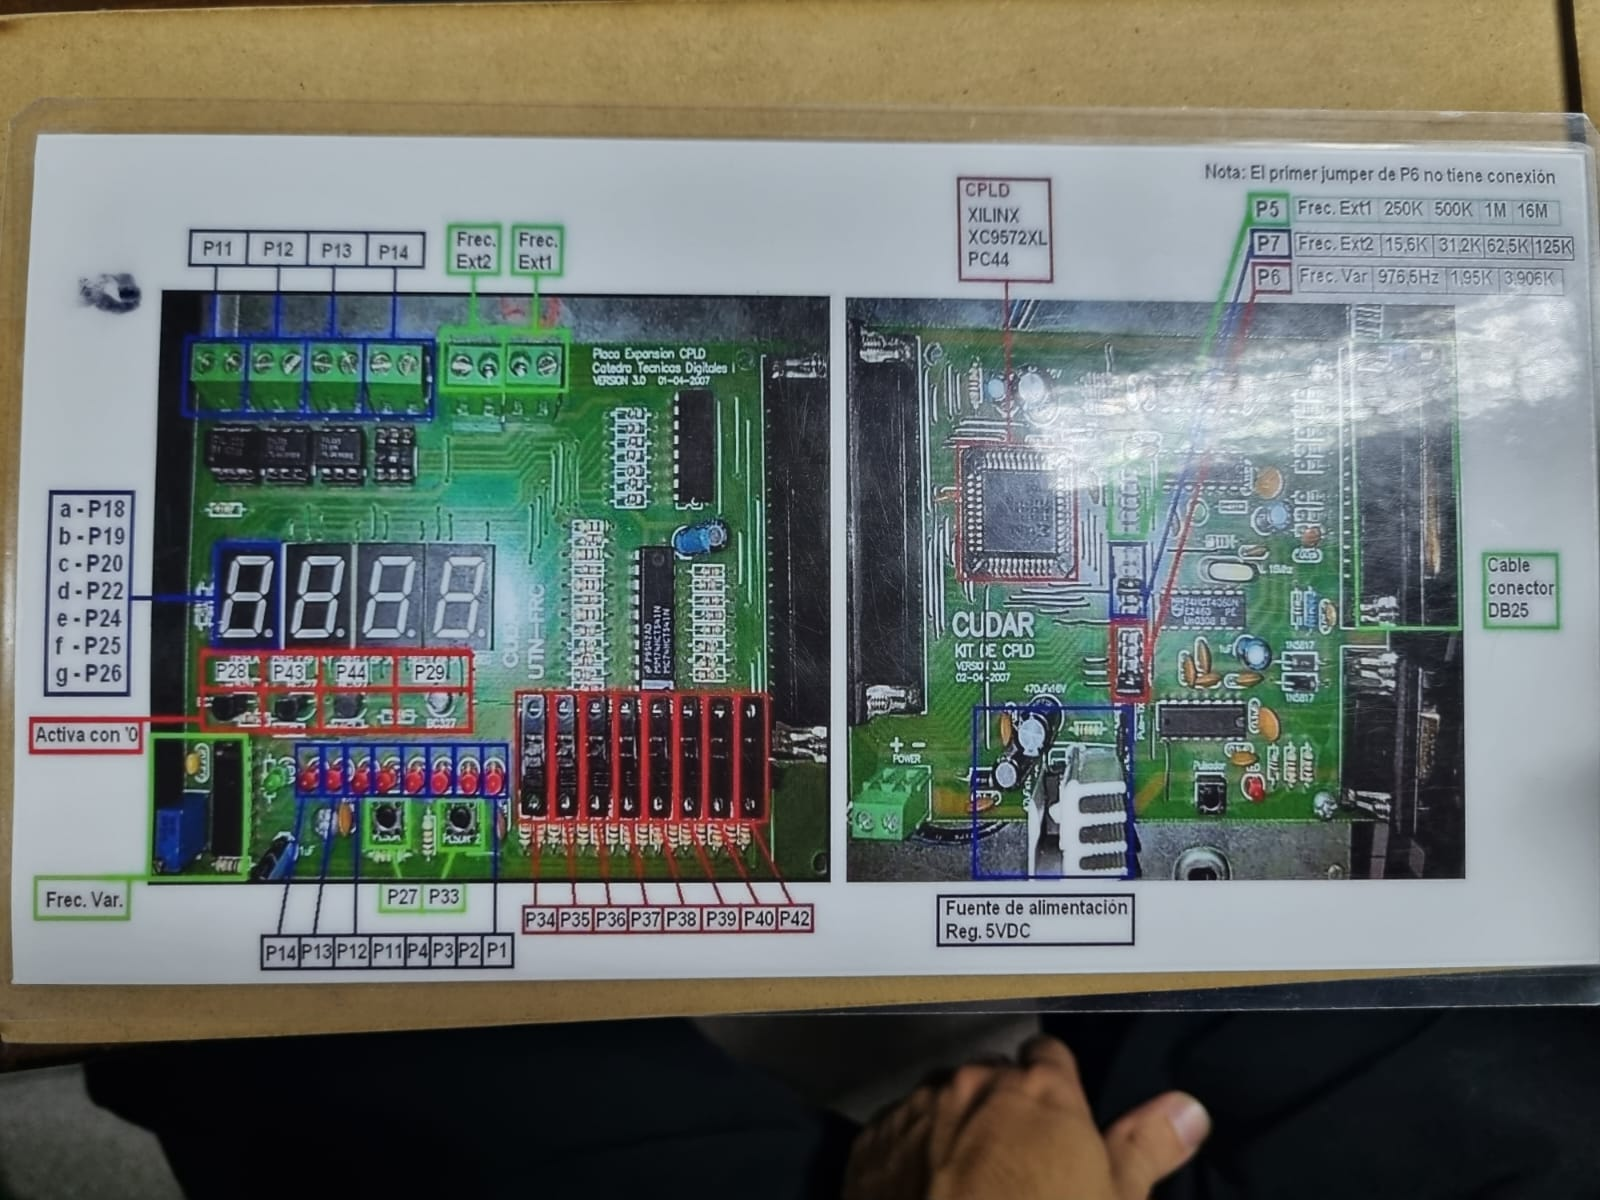
\includegraphics[width=14cm]{./imagenes/diag.jpeg}
\paragraph{Diagrama de disposición de entradas y salidas} En la imagen se puede observar la disposición de cada pin del CPLD XC9572XL marcando cual es su designación numerica. A la hora de cargar el codigo de verilog en el CPLD hay que asignar cual de nuestras salidas o entradas es cada pin del CPLD. En la salidas, se asignaron los segmentos del display según correspondiesen del "a" al "g". Las entradas se asigno: la entrada A al pin 37, la B al pin 36, la C al pin 35 y la D al pin 34, BI al pin 40 y LT al pin 42.
\paragraph{}
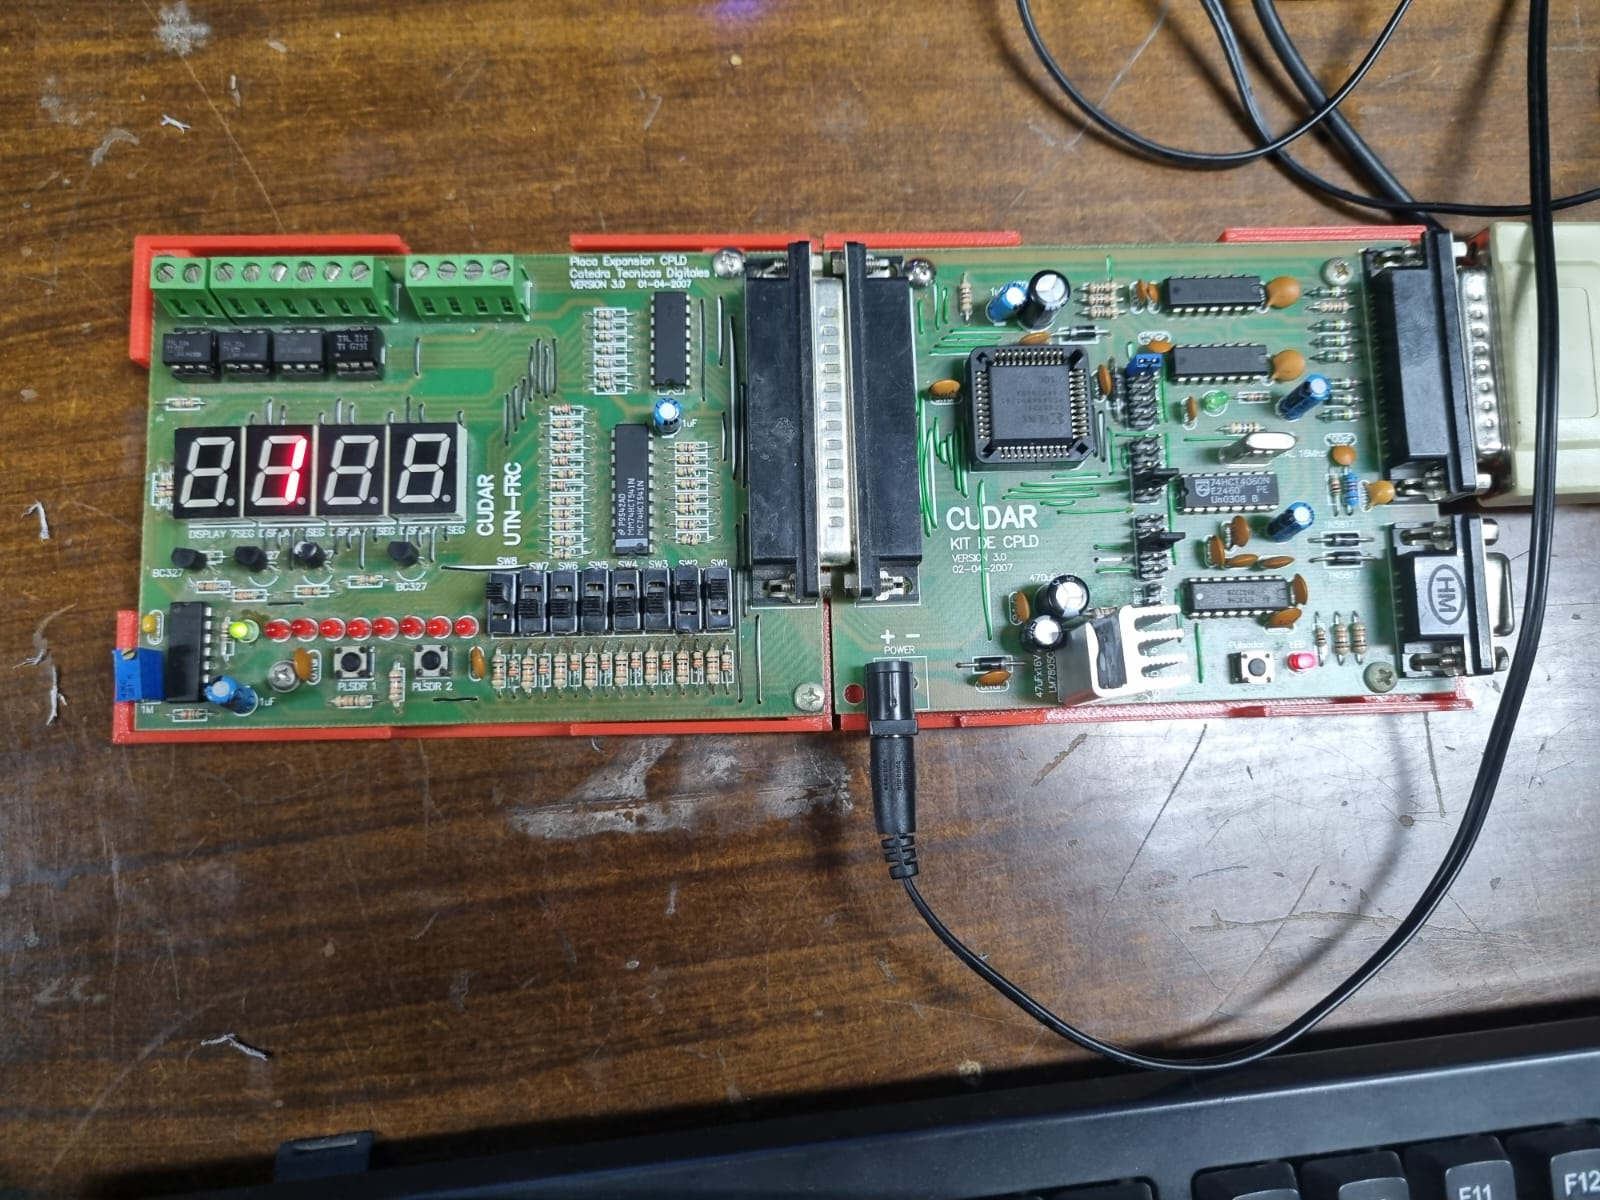
\includegraphics[width=13cm]{./imagenes/uno.jpeg}
\paragraph{}Aqui se muestra la implementación cuando A=1, B=0, C=0 , D=0 , BI=1 y LT=1, lo que corresponde al numero 1 en el display de 7 segmentos.
\paragraph{}
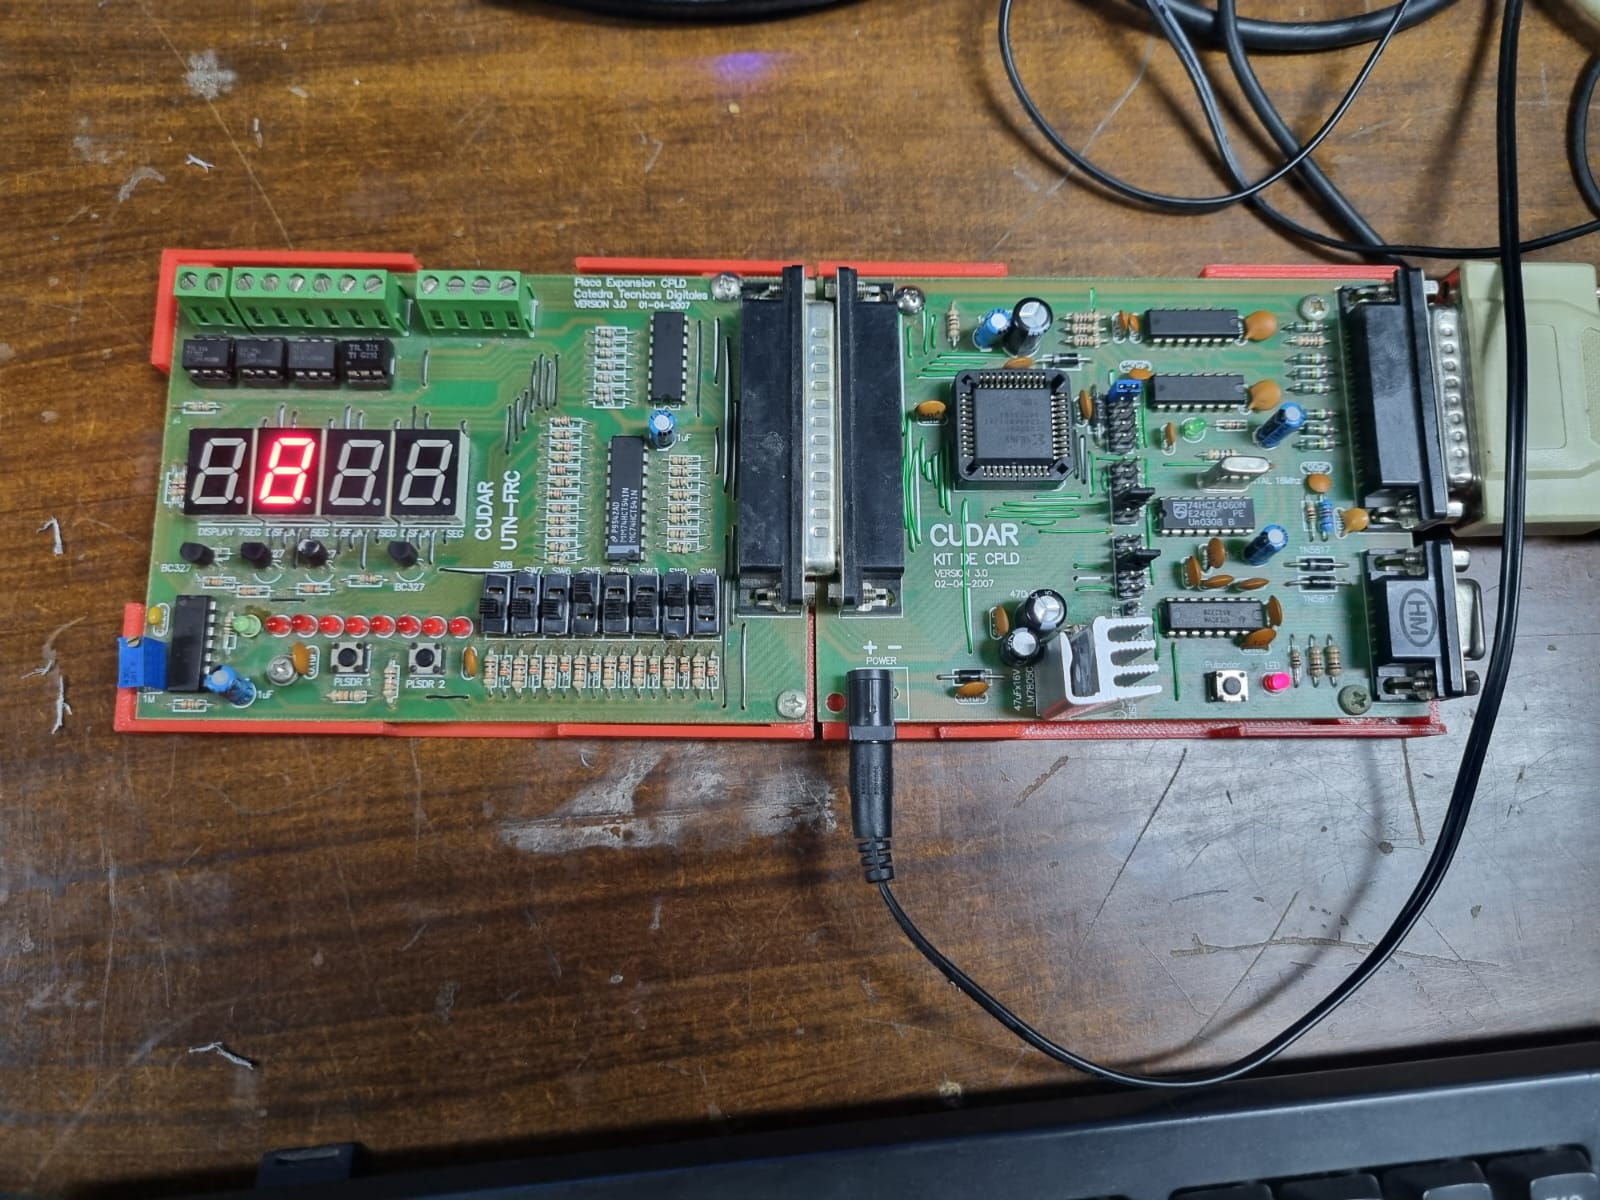
\includegraphics[width=15cm]{./imagenes/ocho.jpeg}
\paragraph{}Aqui se muestra la implementación cuando A=0, B=0, C=0 , D=1 , BI=1 y LT=1, lo que corresponde al numero 8 en el display de 7 segmentos.
